\documentclass[a4paper, 10pt]{article}
\usepackage{amsmath}
\usepackage{fancyhdr}
\usepackage{float}
\usepackage[a4paper, left=0.9in, right=0.9in, top=0.9in, bottom=0.9in]{geometry} % Adjust margins
\usepackage{graphicx}
\usepackage{listings}
\usepackage{matlab-prettifier}

\pagestyle{fancy}

\title{ECE 340 Lab 4}
\author{Omar Mahmoud\\1753607\\Section D21}
\date{11/18/2024}

\lhead{Omar Mahmoud}
\rhead{ECE 340 Lab 4}
\headheight 15pt

\begin{document}

%% Cover Page
\thispagestyle{empty}
\vfill
\maketitle
\vfill

\newpage

% Q1: Reading Audio File
\section{Reading Audio File}
To play and extract the sampling rate, bit-rate, and duration of the the audio file \textit{love\_mono22.wav},
the following MATLAB script was used:
\begin{lstlisting}[style=Matlab-editor, basicstyle=\small\ttfamily]
  %% First few words of love_mono22.wav:
  % I love to love, I love to love you,
  % So much I wanna share and do, wohohoh
  % I love to love, I love to love you,
  % I wanna find a way to you.
  
  [x, Fs] = audioread('love_mono22.wav'); % Fs = sampling rate
  [num_samples, num_channels] = size(x);
  
  % Play the song
  sound(x, Fs);
  
  % Caclulate Bit Rate & Duration
  bits_per_sample = 8;
  bit_rate = Fs * bits_per_sample * num_channels;
  duration = num_samples / Fs;
  
  fprintf('Sampling Rate: %d Hz\n', Fs);
  fprintf('Matrix Size: [%d][%d]\n', num_samples, num_channels);
  fprintf('Bit-Rate: %d bits/sec\n', bit_rate);
  fprintf('Duration: %.2f s\n', duration);
\end{lstlisting}
After running the script the following output was produced providing the requested data:
\begin{lstlisting}[basicstyle=\small\ttfamily]
  Sampling Rate: 22050 Hz
  Matrix Size: [400000][1]
  Bit-Rate: 176400 bits/sec
  Duration: 18.14 s
\end{lstlisting}

% Q2: Audio Spectrum
\section{Audio Specturm}
The DFT of the audio signal was calculated and the first three coefficients where outputed using
the \textit{fft} function in the following MATLAB script:
\begin{lstlisting}[style=Matlab-editor, basicstyle=\small\ttfamily]
  X = fft(x); % Compute the DFT
  fprintf('X[0] = %f + %fi\n', real(X(1)), imag(X(1))); % First coefficient
  fprintf('X[1] = %f + %fi\n', real(X(2)), imag(X(2))); % Second coefficient
  fprintf('X[2] = %f + %fi\n', real(X(3)), imag(X(3))); % Third coefficient
\end{lstlisting}
After running the script the following output was produced:
\begin{lstlisting}[basicstyle=\small\ttfamily]
  X[0] = -16.062500 + 0.000000i
  X[1] = 0.778562 + -0.640574i
  X[2] = 3.169748 + -1.670759i
\end{lstlisting}
\noindent To the scale all the coefficients $X[r]$ by $X'[r] = \frac{X[r]}{\sqrt{N}}$ the following
MATLAB script was used:
\begin{lstlisting}[style=Matlab-editor, basicstyle=\small\ttfamily]  
  N = num_samples; % Total number of samples from section 1
  X_s = X / sqrt(N); % Scale the coefficients
\end{lstlisting}
Then to plot $x[k] = |X'[k]|$ in kHz the following script was used:
\begin{lstlisting}[style=Matlab-editor, basicstyle=\small\ttfamily]
  mag_scaled = abs(X_s); % Magnitude of the DFT
  f_kHz = (0:N-1) * (Fs / N) / 1000; % Frequency in KHz
  mag_dB = 20 * log10(mag_scaled); % Convert to dB
  
  % Plot the magnitude spectrum
  plot(f_kHz(1:floor(N/2)), mag_dB(1:floor(N/2)));
  xlabel('Frequency (kHz)');
  ylabel('Magnitude (dB)');
  title('Magnitude Spectrum of the Audio Signal');
  grid on;
\end{lstlisting}
Which produced the following plot:
\begin{figure}[H]
  \centering
  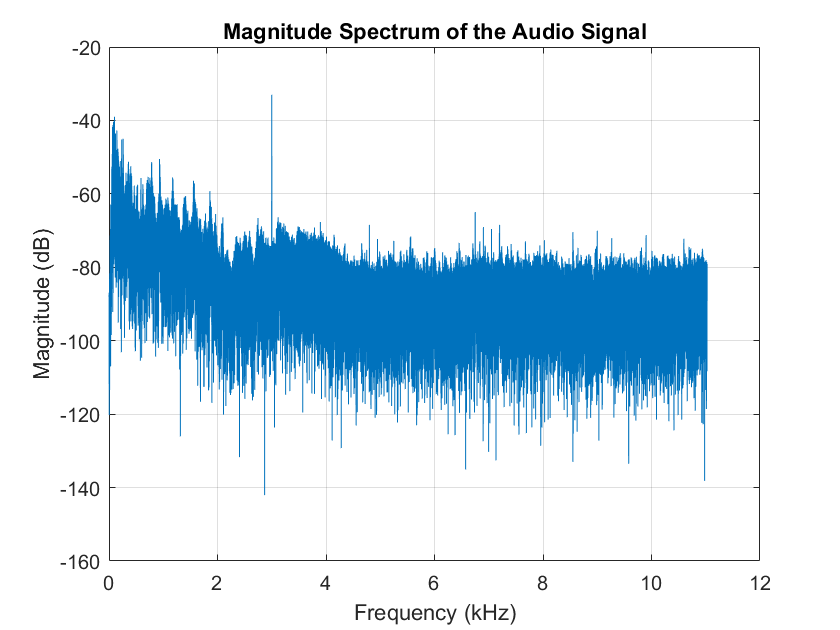
\includegraphics[width=8.5cm]{images/q2d.png}
  \caption{Magnitude specturm of $x[k] = |X'[k]|$.}
\end{figure}
\noindent The plot above depicts the magnitude spectrum of the audio signal from the \textit{love\_mono22.wav} file.
The graph shows prominent peaks caused by variations in the sound signal, likely due to sudden changes
in instrumentals, beats, or lyrics in the song. When we played the song in the previous section, a
consistent ringing sound could be heard in the background. This ringing manifests as a relatively constant
magnitude across the lower intensities. The lower frequencies of the plot (up to ~0.25 kHz) exhibit higher
energy levels, indicating that this song has a strong bass component.

% Q3: Spectrum Estimation
\section{Spectrum Estimation}
To estimate the power spectral density of the signal \textit{love\_mono22.wav} and plot the spectrum
the following MATLAB script was used:
\begin{lstlisting}[style=Matlab-editor, basicstyle=\small\ttfamily]
  N = 512;
  [Px, F] = pwelch(x, N, [], N, Fs);
  plot(F/1000, 10*log10(Px)); %Plots the power spectrum
  %scaling F by 1000 will represent frequency in kHz
  xlabel('Frequency (kHz) ');
  ylabel('Power Spectral Density (in dB) ');
  grid on;
\end{lstlisting}
It produced the following plot:
\begin{figure}[H]
  \centering
  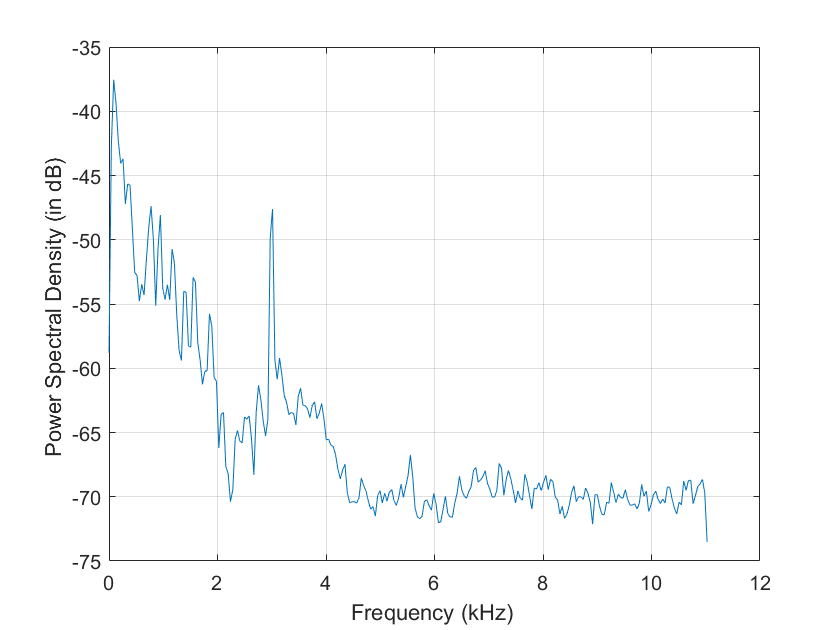
\includegraphics[width=9.5cm]{images/q3a.png}
  \caption{Power Spectral Density Plot of \textit{love\_mono22.wav}.}
\end{figure}
\noindent After examining the power spectral density plot, it is clear that the lower frequencies contain the most 
energy, particularly in the range of 0 kHz to 2 kHz, after which there is a sharp drop with another smaller peak 
between approximately 3 kHz and 4 kHz. The energy peaks slightly above 0 kHz, reaching around -37 dB. Beyond 4 kHz,
the energy levels average out. Going back to the (annoying) noise heard in the audio file, the most likely frequency 
corresponding to it is the sharp spike at approximately 3 kHz mentioned previously.

% Q4: Power Spectrum of 2D Images
\section{Power Spectrum of 2D Images}
Upon inspecting the provided TIF image file, \textit{ayantika.tif}, a very distinct and uniform
grid artifact is visible across the image:
\begin{figure}[H]
  \centering
  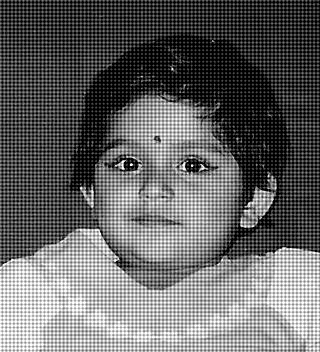
\includegraphics[width=5cm]{images/ayantika.png}
  \caption{ayantika.tif}
\end{figure}
After running the provided 'q4.m' script the following plot was produced:
\begin{figure}[H]
  \centering
  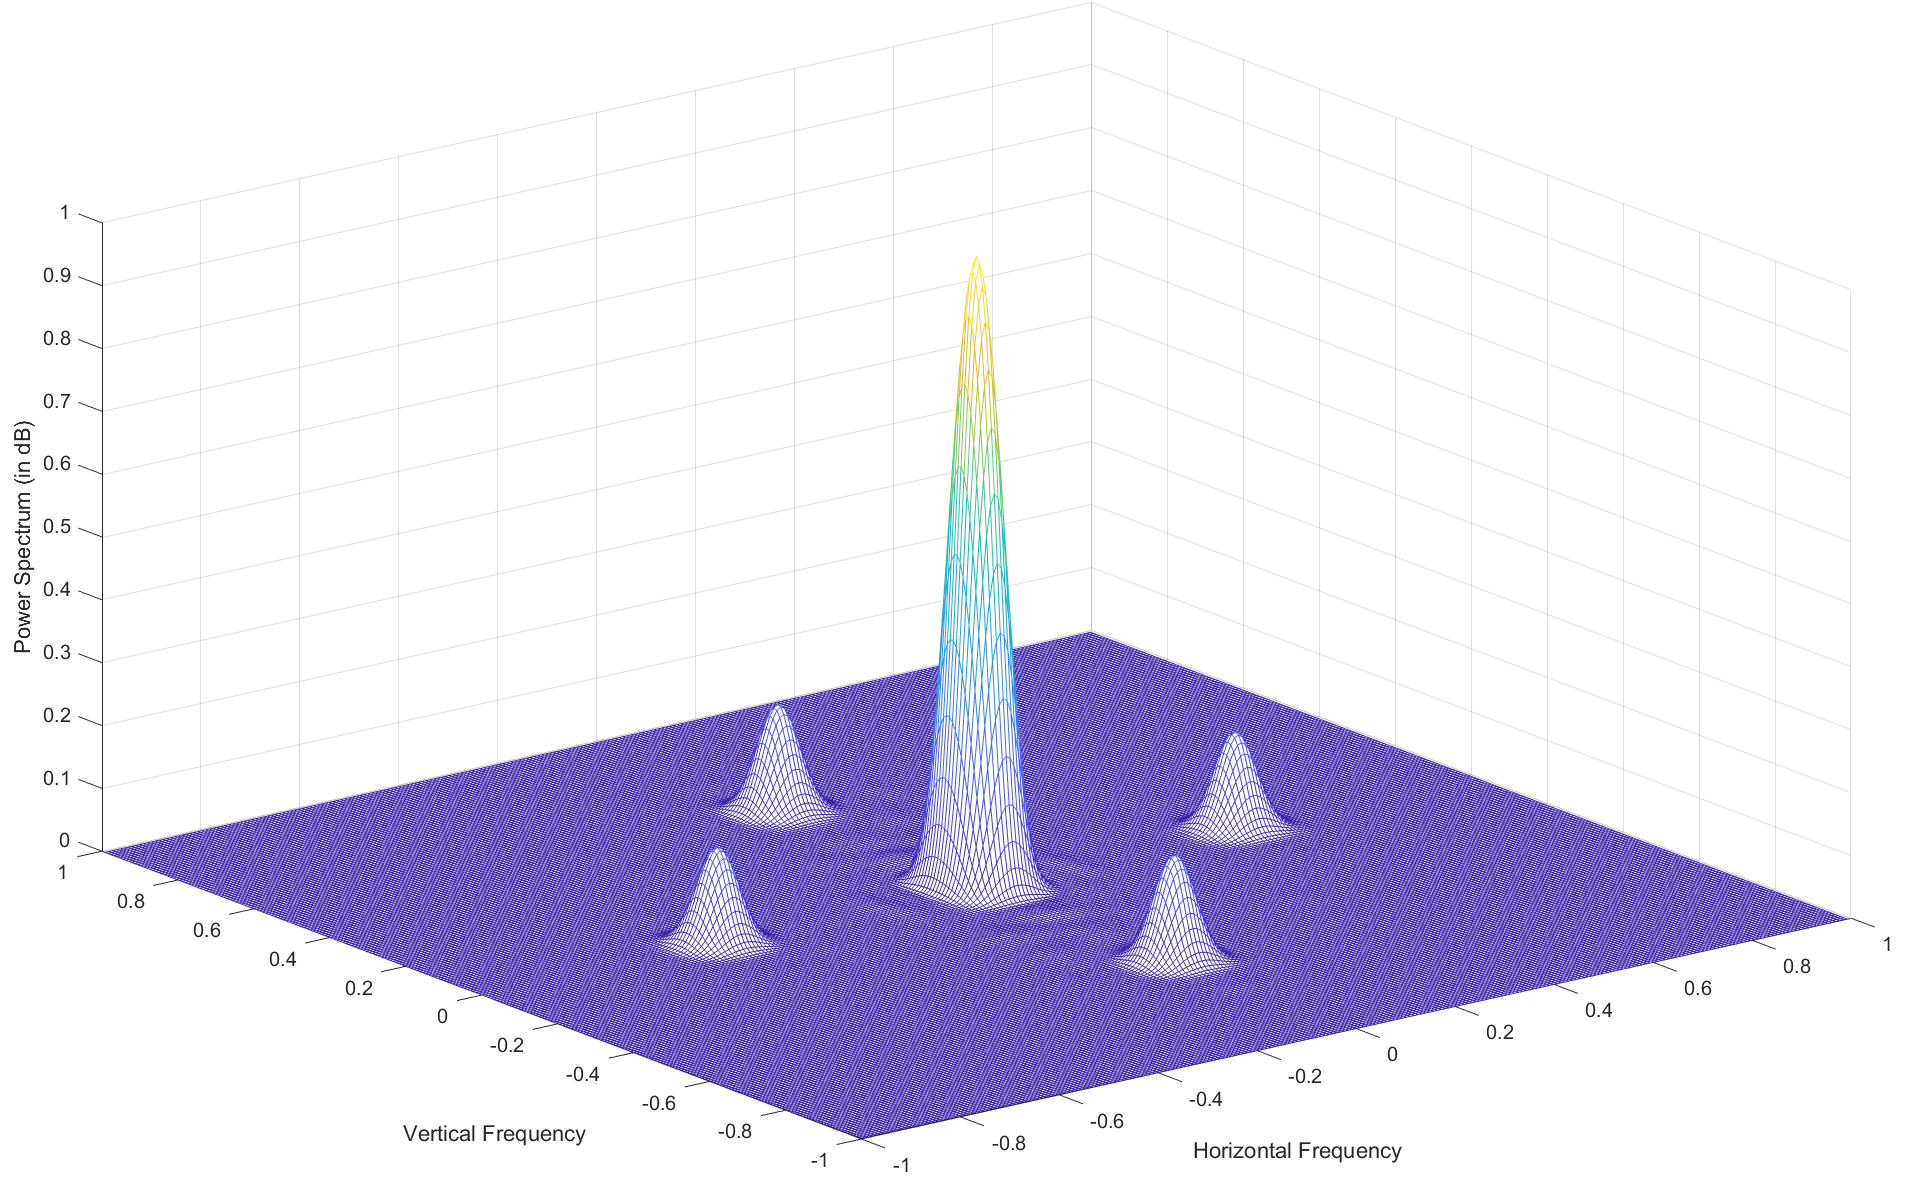
\includegraphics[width=16cm]{images/q4c.png}
  \caption{Spectrum plot produced by 'q4.m'.}
\end{figure}
\noindent By examining the plot, the main lobe is found to peak at (0, 0, 1). Then the four other peaks are located at 
(-0.5, 0, 1.5), (0, -0.5, 1.7), (0.5, 0, 1.5), and (0, 0.5, 1.7).
\end{document}